\documentclass[hyperref={bookmarks=true, unicode=true, colorlinks=true, plainpages=false, pdfkeywords={Skaut, Junak, Skauting, Vychovna metoda}, linkcolor=OrangeRed, anchorcolor=OrangeRed, citecolor=RawSienna, filecolor=RawSienna, menucolor=OrangeRed, urlcolor=RawSienna, pdftex}, compress, xelatex, xcolor=dvipsnames, print]{beamer}
% Nastavení vzhledu
\useinnertheme[shadow]{rounded}
\usecolortheme{wolverine}
\setbeamertemplate{itemize subitem}[triangle]
\setbeamertemplate{headline} {
  \hbox{
  \begin{beamercolorbox}[wd=0.5\paperwidth, ht=2.65ex, right]{section in head/foot}
    \insertsectionnavigationhorizontal{.5\paperwidth}{\hskip0pt plus1fill}{\hskip0pt plus1fill}
  \end{beamercolorbox}
  \begin{beamercolorbox}[wd=0.5\paperwidth, ht=2.65ex, left]{subsection in head/foot}
    \insertsubsectionnavigationhorizontal{0.5\paperwidth}{}{\hfill\hfill}
  \end{beamercolorbox}}
  }
\setbeamertemplate{footline} {
  \hbox{
    \begin{beamercolorbox}[wd=0.333333\paperwidth, ht=2.25ex, center]{author in head/foot}
      \usebeamerfont{author in head/foot}\insertshortauthor~(\insertshortinstitute)
    \end{beamercolorbox}
    \begin{beamercolorbox}[wd=0.333333\paperwidth, ht=2.25ex, center]{title in head/foot}
      \usebeamerfont{title in head/foot}\insertshorttitle
    \end{beamercolorbox}
    \begin{beamercolorbox}[wd=0.333333\paperwidth, ht=2.25ex, center]{date in head/foot}
      \usebeamerfont{date in head/foot}\insertshortdate{}\hspace*{1em}\insertframenumber{}/\inserttotalframenumber
    \end{beamercolorbox}
    }
  }
% Další balíčky a nastavení
\usepackage{xltxtra}
\usepackage{xunicode}
\usepackage{polyglossia}
\setdefaultlanguage{czech}
\usepackage{multicol}
\author{Vojtěch Zeisek}
\institute[Junák --- český skaut]{Ekologický odbor Výkonné rady Junáka --- českého skauta, z.~s.\\
Katedra botaniky Přírodovědecké fakulty UK \&~Botanický ústav AV ČR, v.~v.~i.}
\title{Skautská výchovná metoda}
\subtitle{A~její proměny za poslední století a~desetiletí}
\date{KDF MFF UK 15. 4. 2015}
\titlegraphic{
\includegraphics[width=2cm]{lilie.png}}

\begin{document}

\begin{frame}
\titlepage
\end{frame}

\section{Úvod}

\subsection{Z~historie}

\begin{frame}{Jak to začalo --- velmi stručná historie světového skautingu}
\begin{itemize}
 \item Skautské hnutí založil generál Robert Stephenson Smyth Baden-Powell, pozdější Lord of Gilwell, 1857--1941
 \item Nepřijat na Oxford, 1876 nastupuje na vojenskou akademii a~odjíždí do Indie
 \item Kreslil, hrál divadlo, psal do novin, učil se hindsky, inspiruje se místními stopaři a~zakládá průzkumné oddíly (scouts)
 \item 1887 připlouvá do Jižní Afriky, převelen ke zpravodajské službě, mj. mapuje Dračí hory, \alert{sepisuje příručku pro vojenské průzkumníky} (o~pohybu v~přírodě --- inspirace pro děti),~\ldots
 \item 1899--1900 úspěšně brání obležený Mafeking před Búry, povýšen na generálmajora, národní hrdina
 \item Žádá o~propuštění z~armády, 1907 1. skautský tábor (Brownsea Island), píše Scouting for Boys (1908)
 \item 1920 1. světové Jamboree v~Londýně
\end{itemize}
\end{frame}

\begin{frame}{Robert Baden-Powell}{Co hlavního si mladý důstojník odnesl ze školy\ldots}
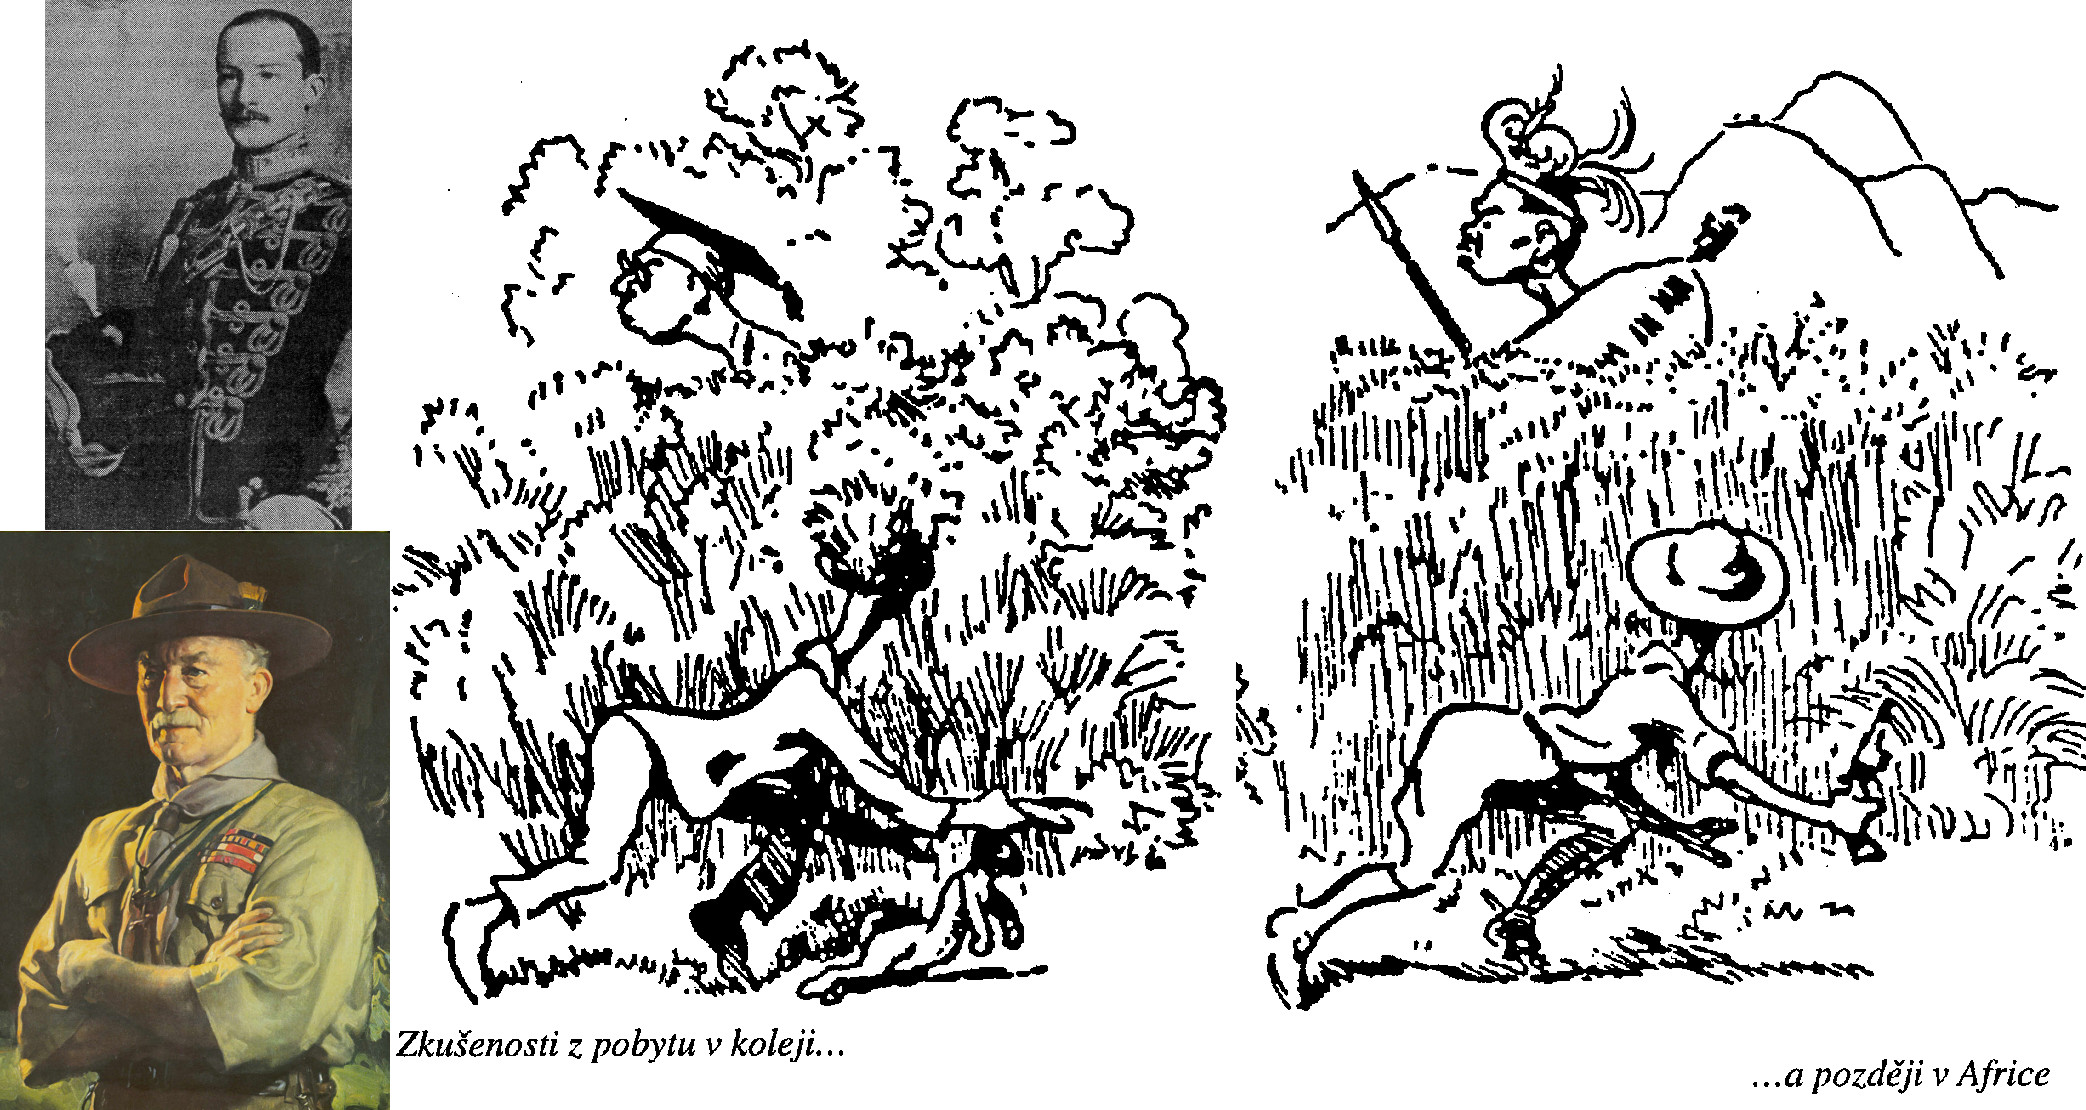
\includegraphics[width=\textwidth]{bp.jpg}
\end{frame}

\begin{frame}{Ernest Thompson Seton (1860--1946) --- woodcraft a~vliv na český skauting 1}
\begin{multicols}{2}
  \begin{center}
    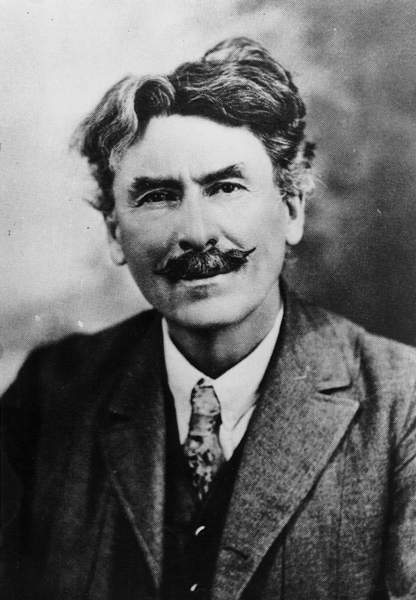
\includegraphics[height=6cm]{seton.jpg}
  \end{center}
\columnbreak
\begin{itemize}
 \item Původně anglický malíř, spisovatel, učitel a~přírodovědec
 \item Pracoval v~muzeu, živil se i~psaním knih
 \item Skvělý pozorovatel a~vypravěč o~životě zvířat
 \item Většinu času trávil v~divoké přírodě v~USA, učil se od Indiánů jejich praktickým znalostem a~dovednostem i~filozofii a~pohledu na svět
\end{itemize}
\end{multicols}
\end{frame}

\begin{frame}{Ernest Thompson Seton --- woodcraft a~vliv na český skauting 2}
\begin{itemize}
 \item 1902 založil \textit{Woodcraft Indians} --- hnutí inspirující se životem Indiánů (znalosti a~respekt k~přírodě, příroda a~krajina jako zdroj duchovní inspirace, fyzická zdatnost, rukodělné práce, zručnost, morální kodex) snažící se o~výchovu a~poznání
 \item S~americkou skautskou organizací se rozešel ve zlém, s~Baden-Powellem vycházel velice dobře
 \item Trochu nespravedlivě ve stínu skautingu, jeho hnutí je mnohem menší než to skautské, vzájemně se ovlivňovaly
 \item Mnoha společných prvků se skautingem (práce v~malých skupinách, učení se od ostatních apod.)
 \item Knihy E.~T. Setona měly velký vliv na zakladatele českého skautingu, dále u~nás působí \href{http://www.woodcraft.cz/}{Liga lesní moudrosti} (ta přímo navazuje na jeho americké hnutí)
\end{itemize}
\end{frame}

\begin{frame}{Velmi stručná historie českého skautingu~1}
\begin{itemize}
 \item Založil jej pražský učitel tělocviku Antonín Benjamín Svojsík, 1876--1938
 \item 1909 se dozvěděl o~skautingu, 1911 se vydal do Anglie
 \item Ve školním roce 1911/12 založil na žižkovské reálce 1.~skautskou družinu, reakce veřejnosti byla chladná
 \item 1912 sepisuje \alert{Základy junáctví}, konzultuje své myšlenky s~intelektuální elitou doby (Drtina, Masaryk, Kramář, Aleš, Jirásek, Rais, Guth-Jarkovský,~\ldots)
 \item 1912 1. skautský tábor u~Lipnice nad Sázavou (šli tam pěšky)
 \item 1918 skauti pro revoluční Národní výbor zajišťovali kurýrní službu (a~vydávali 1.~známky RČS)
 \item 1919 založen Svaz junáků --- skautů RČS
 \item Vznikla řada skautských organizací
 \item 1939 se skautské organizace spojily do Junáka --- svazu skautů a~skautek RČS
\end{itemize}
\end{frame}

\begin{frame}{Antonín Benjamín Svojsík a~první čeští skauti}
\begin{flushright}
Kolorované fotografie z~tábora 1912\\
\end{flushright}
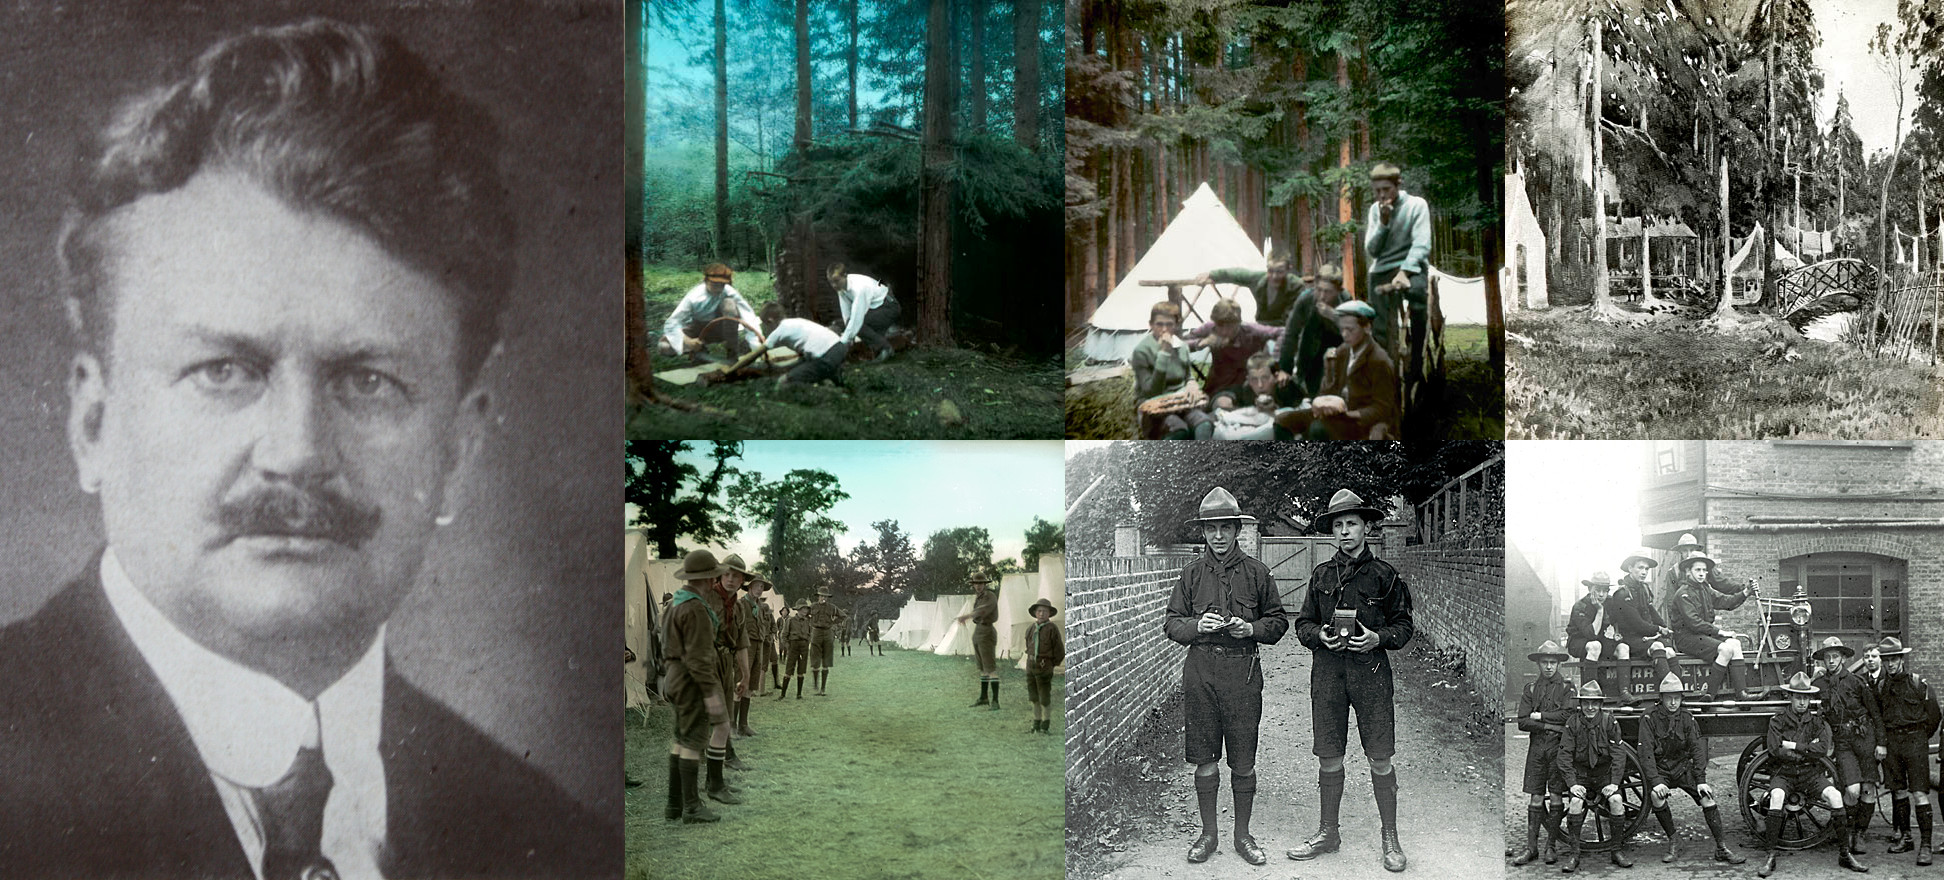
\includegraphics[width=\textwidth]{svojsik_prvni_skauti.jpg}
\begin{flushright}
Snímky pravděpodobně z~20. let\\
\end{flushright}
\end{frame}

\begin{frame}{Velmi stručná historie českého skautingu~2}
\begin{itemize}
 \item Za války se skauti zapojili do odboje, zahraničních armád
 \item 1940 Gestapo rozehnalo řadu táborů, zatýkání představitelů, rozpuštění Junáka (obnoven 1945)
 \item Ihned po únoru 1948 komunisti obsadili ústředí Junáka, vytvořen akční výbor, Junák zlikvidován
 \item 1949 měly vznikat pionýrské oddíly, 1950 Junák formálně zrušen (fakticky už neexistoval)
 \item V~50. letech bylo mnoho skautských činovníků odsouzeno
 \item 1968 Junák obnoven
 \item 1969 ÚV KSČ rozhodlo o~vzniku Svazu socialistické mládeže (SSM), 1970 Junák násilně včleněn do SSM
 \item V~70. a~80. letech řada oddílů přežívala pod hlavičkou jiných organizací v~rámci SSM
 \item 1989 obnova Junáka, v~90. letech probíhaly debaty o~identitě a~budoucím směřování
\end{itemize}
\end{frame}

\subsection{Myšlenkové základy --- špetka filozofie}

\begin{frame}{Poslání Junáka}
\begin{center}
\begin{Large}
Posláním Junáka je \textbf{podporovat rozvoj osobnosti} mladých lidí, jejich \textbf{duchovních, mravních, intelektuálních, sociálních a~tělesných schopností} tak, aby byli po celý život připraveni plnit povinnosti k~sobě samým, bližním, vlasti, přírodě a~celému lidskému společenství \textbf{v~souladu s~principy a~metodami}, stanovenými zakladatelem skautského hnutí, lordem Robertem Baden-Powellem a~zakladatelem českého skautingu, prof. Antonínem Benjamínem Svojsíkem.
\end{Large}
\end{center}
\begin{itemize}
\item Za 1. republiky se na tvorbě skautské metodiky podílely tehdejší špičky psychologie, pedagogiky a~dalších oborů.
\end{itemize}
\end{frame}

\begin{frame}{Principy skautského hnutí}
\begin{enumerate}
\item \textbf{Povinnost k~Bohu}, chápaná jako povinnost hledat v~životě \textbf{vyšší hodnoty než materiální};
 \begin{itemize}
 \item Jde o~morálku, slušnost, dobrotu --- ne nutně o~víru
 \end{itemize}
\item \textbf{povinnost vůči ostatním}, chápaná jako věrnost své vlasti, která je v~souladu s~úsilím o~mír, o~vzájemné pochopení a~spolupráci mezi lidmi, národy a~různými sociálními skupinami; je pojata jako \textbf{závazek účastnit se na rozvoji společnosti, jako úcta a~láska prokazovaná bližním a~přírodě};
 \begin{itemize}
 \item Nejsme tu jen sami za sebe, ale jsme součástí širšího společenství, na jehož běhu se chceme aktivně podílet, díky své moci máme zodpovědnost za osud světa
 \end{itemize}
\item \textbf{povinnost vůči sobě}, chápaná jako odpovědnost za \textbf{rozvoj sebe sama}.
 \begin{itemize}
 \item Nesmíme zapomínat ani na sebe (včetně odpočinku:-)
 \end{itemize}
\end{enumerate}
\end{frame}

\begin{frame}{Skautský slib a~zákon}
\begin{multicols}{3}
\textbf{Slib}

Slibuji na svou čest, jak dovedu nejlépe: sloužit nejvyšší Pravdě a~Lásce věrně v~každé době, plnit povinnosti vlastní a~zachovávat zákony skautské, duší i~tělem být připraven pomáhat vlasti i~bližním.\\
\textit{Dodatek pro věřící:} K~tomu mi dopomáhej Bůh.\\
\columnbreak
\textbf{Heslo}\\ Buď připraven!\\
\vfil
\textbf{Zákon}\\
Skaut je
\begin{enumerate}
 \item pravdomluvný
 \item věrný a~oddaný
 \item prospěšný a~pomáhá jiným
 \item přítelem všech lidí dobré vůle a~bratrem každého skauta
\end{enumerate}
\columnbreak
\begin{enumerate}
 \setcounter{enumi}{4}
 \item zdvořilý
 \item ochráncem přírody a~cenných výtvorů lidských
 \item poslušný rodičů, představených a~vůdců
 \item veselé mysli
 \item hospodárný
 \item čistý ve slovech, myšlení a~skutcích
\end{enumerate}
\end{multicols}
\end{frame}

\begin{frame}{Cíl skautské výchovy}
\begin{itemize}
 \item Základní vodítko: principy a~poslání skautského hnutí, skautský slib a~zákon
 \item Výchovné cíle
 \begin{itemize}
  \item Musí být v~souladu se skautskými hodnotami
  \item Musí být praktické --- připravit děti na reálný život
  \begin{itemize}
   \item Neznáme budoucnost
  \end{itemize}
  \item Mohou jít proti mainstreamu --- televize,~\ldots
 \item Děti v~oddíle děti průměrně tráví pár hodin týdně na schůzce a~jednou za pár týdnů den/víkend na výpravě --- abychom je mohli pozitivně ovlivnit, musíme tento krátký (oproti škole, rodině) čas využít maximálně efektivně
 \end{itemize}
 \item Musí to děti bavit
 \begin{itemize}
 \item „Ryby je nutné lovit na to, co chutná rybám a~ne na to, co chutná rybáři.“ (Baden-Powell)
 \end{itemize}
 \item Tvrdíme, že máme morální právo ovlivňovat hodnotový žebříček dětí směrem, který považujeme za správný
\end{itemize}
\end{frame}

\section{Metodika}

\subsection{Výchovná metoda}

\begin{frame}{Skautská výchovná metoda\ldots}
\ldots vede mladého člověka na cestě osobního růstu: soustava výchovy a~sebevýchovy vedoucí k~upevňování charakteru, tvorbě hodnotového systému a~rozvoji dovedností a~znalostí:
\begin{itemize}
 \item \textbf{Slib a~zákon} --- sebevýchova, dobrovolný závazek
 \item \textbf{Učení se zkušeností} --- praktická i~mravní výchova
 \item \textbf{Družina} --- schopnost být platným členem společenství
 \item \textbf{Symbolický rámec} --- přitažlivé, inspirující a~obohacující
 \item \textbf{Příroda} --- výchovné prostředí, předmět zájmu, ochrany i~citového a~duchovního rozvoje
 \item \textbf{Program osobního růstu} --- pestrý, přitažlivý program i~všestranný individuální rozvoj
 \item \textbf{Dospělí průvodci} --- dospělí ukazují cestu, pomáhají, podporují a~povzbuzují s~respektem k~jedinečnosti dítěte
\end{itemize}
\begin{tiny}(Definovaná \href{http://krizovatka.skaut.cz/stredisko/novy-obcansky-zakonik-stanovy/nove-stanovy}{ve stanovách}, rozpracovaná v~\href{http://krizovatka.skaut.cz/oddil/program/skauti-skautky}{metodických materiálech})\end{tiny}
\end{frame}

\begin{frame}{Historické podoby skautské výchovné metody~1}
\begin{multicols}{2}
\textit{Základy junáctví}, Svojsík, 1912, 1921, reprint 1991
\begin{itemize}
 \item Pobyt v~přírodě
 \item Umění pozorovati
 \item Táboření
 \item Noclehování v~přírodě
 \item Škola práce a~rytířství
 \item Fyzický vývoj a~vliv organizace
 \item (Vycházel ze \textit{Scouting for Boys} (Baden-Powell, 1908, česky 2009, \textit{Skauting pro chlapce}), knih Setona a~českých specifik)
\end{itemize}
\columnbreak
\textit{Aids to Scoutmastership}, Baden-Powell, 1920, česky 2006 (\textit{Na pomoc skautským vůdcům})
\begin{itemize}
 \item Charakterové vlastnosti
 \item Zdraví a~zdatnost
 \item Rukodělné práce a~řemeslné dovednosti
 \item Služba druhým
\end{itemize}
\begin{center}
 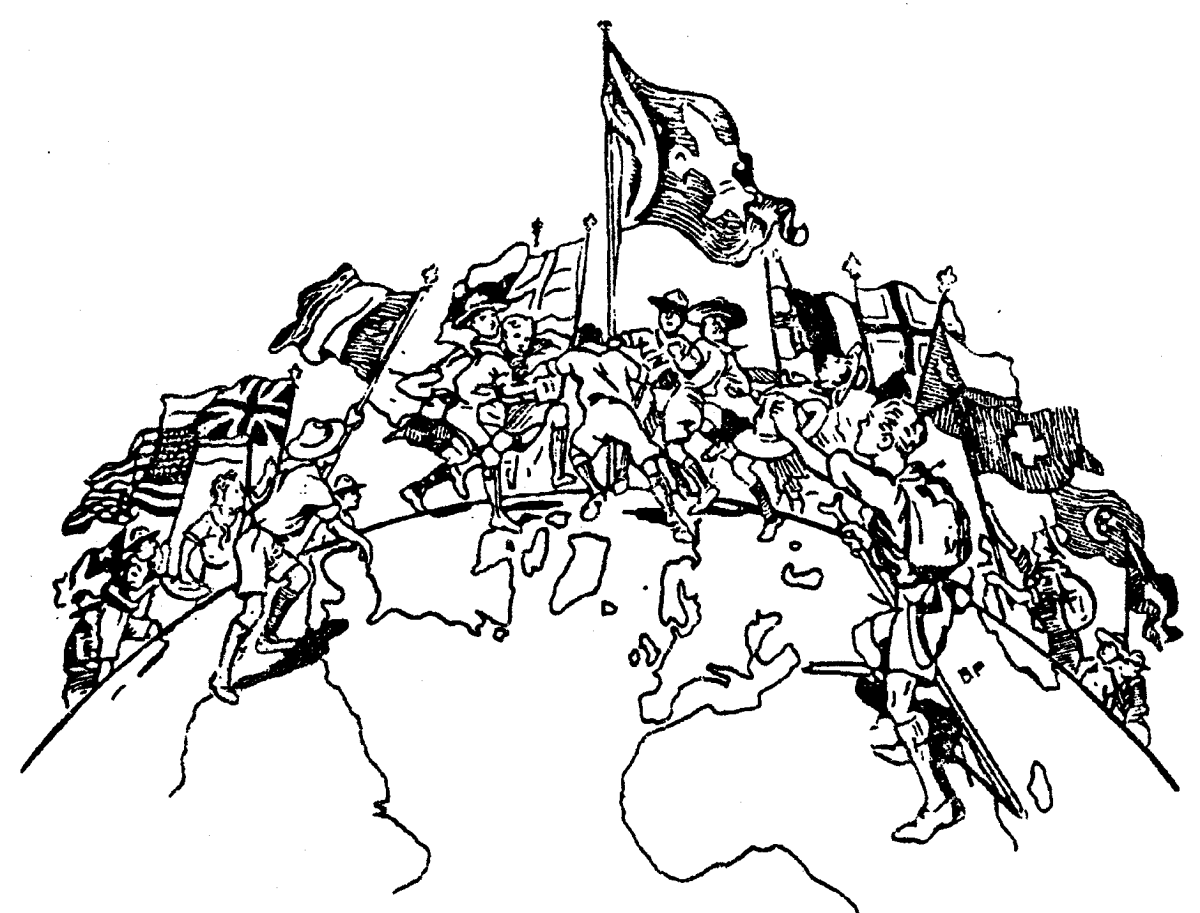
\includegraphics[width=3cm]{sireni.png}
\end{center}
\end{multicols}
\end{frame}

\begin{frame}{Historické podoby skautské výchovné metody~2}
\begin{multicols}{2}
World Organisation of Scout Movement, 1977\\
\begin{footnotesize}
\href{http://www.scout.org/node/65}{http://www.scout.org/node/65}
\begin{center}
 
\includegraphics[width=2cm]{wosm.jpg}
\end{center}
\begin{itemize}
 \item Slib a~zákon
 \item Učení se zkušeností
 \item Členství v~malých skupinách
 \item Postupný a~stimulující program
\end{itemize}
\end{footnotesize}
\columnbreak
Junák, do 2014
\begin{itemize}
\begin{footnotesize}
\item Skautský slib a~zákon
\item Učení se prostřednictvím praktických činností a~her
\item Týmová práce ve skupinkách
\item Zájem a~spoluúčast každého mladého člověka na jeho osobním rozvoji
\item Symbolický rámec
\item Pobyt a~činnost v~přírodě, její poznávání a~ochrana
\item Podpora mladých lidí dospělými
\item Služba společnosti
\item Postupně stimulující programy
\item Symbolika a~výchovné prostředí
\end{footnotesize}
\end{itemize}
\end{multicols}
\end{frame}

\subsection{Čas na změnu}

\begin{frame}{Proč nový program?}
\begin{itemize}
\item Změna dnešní společnosti
 \begin{itemize}
 \item konzum, zrychlená doba, vliv médií, internetu, techniky,~\ldots
 \item děti rychleji dospívají a~baví je jiné věci než v~minulosti
 \end{itemize}
\item Historický vývoj Junáka (zákazy,~\ldots) --- od 1. republiky do přelomu tisíciletí se moc nezměnil
\item Charta českého skautingu (2005) --- obecné cíle rozvoje
 \begin{itemize}
 \item Odkazuje na historické kořeny, uvědomuje si současný svět a~otevírá skauting pro budoucnost
 \end{itemize}
\end{itemize}
\begin{center}
\begin{tabular}{| l | l |}
\hline
{\textbf{„Starý program“}} & {\textbf{„Nový program“}}\\
\hline\hline
Jednotlivé dílčí úkoly & Komplexní úkoly, projekty\\
\hline
Hlavně o~znalostech & Něco dokázat, udělat\\
\hline
Stejná úroveň pro všechny & Nastavitelná obtížnost\\
\hline
Sám o~sobě neatraktivní, & Provázaný, moderní,\\
bez kontextu a~návaznosti & motivační, atraktivní\\
\hline
\end{tabular}
\end{center}
\end{frame}

\subsection{Program}

\begin{frame}{Výchovný program}
\begin{itemize}
\item Výsledek skautské výchovy --- výchovné cíle skautingu
 \begin{itemize}
 \item Mladý člověk cca na konci střední až počátku vysoké školy
 \item Dovednosti, schopnosti a~postoje, které má mladý člověk ovládat --- koho chceme vychovat
 \end{itemize}
\item Skautská metoda
\item Věkové kategorie
\item Výchovné nástroje
\item Metodické příručky pro vedoucí
\item Hodnocení kvality oddílu a~výchovného dopadu
\item Management, lidské zdroje, found rising,~\ldots
\item Reforma výchovného programu: 2005--2013
\begin{itemize}
 \item Vlastně nikdy nekončí\ldots~(stále je dost práce\ldots)
\end{itemize}

\end{itemize}
\end{frame}

\begin{frame}{Jak při tvorbě nového výchovného programu postupujeme}
\begin{enumerate}
\item Definování obecných cílů (kompetence)
\item Rozpracování dílčích cílů (podle věku,~\ldots)
\item Výběr vhodných indikátorů (jak poznáme, je-li cíl splněn)
\item Tvorba programů vedoucích ke splnění cílů
\end{enumerate}
\begin{itemize}
\item Obecné cíle se definovaly na začátku pro všechny věkové kategorie
\item Rozpracování obecných cílů se provádí pro jednotlivé věkové kategorie (dílčí cíle)
\item Další nástroje sloužící k~motivaci,~\ldots
\item Postupná tvorba databáze programů
\item Metodická podpora pro vedoucí a~další „uživatelská“ podpora vedoucím oddílů ze strany organizace
\end{itemize}
\end{frame}

\begin{frame}{Co chceme, aby uměl mladý člověk poté, co projde naší výchovou a~na prahu dospělosti odejde?}
\begin{center}
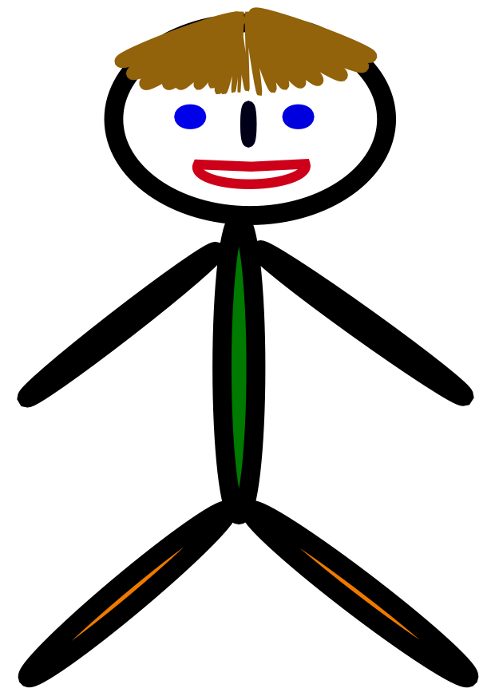
\includegraphics[height=6.5cm]{pepicek.png}
\end{center}
\end{frame}

\subsection{Kompetence}

\begin{frame}{Skauting a~klíčové kompetence}
\begin{center}
Klíčové kompetence: přenosný a~univerzálně použitelný \textbf{soubor vědomostí, dovedností a~postojů}, které potřebuje každý jedinec \textbf{pro své osobní naplnění a~rozvoj, pro zapojení se do společnosti} a~úspěšnou zaměstnatelnost.
\end{center}
\begin{itemize}
\item Kompetence je souborem schopností, dovedností, znalostí a~postojů vztahující se k~určité oblasti
\item Kompetence se rovnají výchovným záměrům
\item Jsou rozpracované pro jednotlivé kategorie
\item Navazují na ně výchovné cíle a~metody
\item Úspěšnost definují indikátory (ukazatele, zda dochází k~rozvoji dané kompetence)
\item Jsou zpracovávány a~konzultovány s~odborníky na danou oblast (i~mimo Junáka)
\end{itemize}
\end{frame}

\begin{frame}{Seznam kompetencí}
\begin{enumerate}
\item Duchovní kompetence
 \begin{itemize}
 \item Láska, svědomí, meditace, globální zodpovědnost
 \item V~podstatě jde o~morálku v~nejširším smyslu
 \end{itemize}
\item Psychologické (vztahové)
 \begin{itemize}
 \item Já (k~sobě), já a~ty, já a~my, já a~společnost
 \item Sociální dovednosti, začlenění se do společnosti
 \end{itemize}
\item Manažerské
 \begin{itemize}
 \item Sám sobě manažerem, práce s~informacemi a~řešení problému, vlastní názor, odolávání manipulaci, prezentace na veřejnosti, týmová práce, komunikace
 \end{itemize}
\item Občanské (enviromentální)
 \begin{itemize}
 \item Krása -- vnímání a~vytváření, krása a~jedinečnost přírody, vztah k~přírodě, vztah ke krajině, vědomí provázanosti, respekt k~různosti, aktivní občan
 \item Ochrana přírody díky lásce k~ní, aktivní přístup ke světu
 \end{itemize}
\item Praktické dovednosti
 \begin{itemize}
 \item Přežití v~přírodě, osobní dovednosti, společenské dovednosti, řešení krizových situací
 \end{itemize}
\end{enumerate}
\end{frame}

\begin{frame}{Příklad rozpracování jedné kompetence}
\begin{itemize}
\item Kompetence
 \begin{itemize}
 \item Má dovednosti a~nástroje pro praktický život, umí použít „pracovní nástroje“ své doby (politické, finanční, mediální\ldots)
 \end{itemize}
\item Výchovný cíl
 \begin{itemize}
 \item Dokáže hospodařit s~penězi (8--10 let)
 \end{itemize}
\item Metody
 \begin{itemize}
 \item Hry, ve kterých jsou použity peníze pro nákup potřebných surovin („budovatelské strategie“,~\ldots)
 \item Nakupování potravin a~jiných věcí pro oddíl
 \item Vedení pokladny družiny, vybírání peněz na výpravě
 \end{itemize}
\item Indikátory
\begin{itemize}
 \item Šetří si nějaké peníze se svého kapesného
 \item Nekupuje si zbytečnosti
 \item Bezchybně vrátí peníze po nákupu
\end{itemize}
\end{itemize}
\end{frame}

\section{Stezka}

\begin{frame}{Oblasti stezky}
\begin{itemize}
\item Moje dovednosti a~znalosti
 \begin{itemize}
 \item Praktický život, fyzická zdatnost, buď připraven, hledání řešení, vyjadřování, zručnost
 \end{itemize}
\item Kdo jsem?
 \begin{itemize}
 \item Já a~můj život, moje svědomí, osobní rozvoj
 \end{itemize}
\item Můj kamarád
 \begin{itemize}
 \item Vztahy mezi lidmi, moje vztahy, komunikace mezi lidmi, pomoc druhým
 \end{itemize}
\item Můj domov
 \begin{itemize}
 \item Moje rodina, moje parta, družina jako tým
 \end{itemize}
\item Svět okolo nás
 \begin{itemize}
 \item Já a~demokracie, já občan, propojený svět, různost světa, příběhy našeho světa
 \end{itemize}
\item Příroda kolem nás
 \begin{itemize}
 \item Pobyt v~přírodě, vnímání přírody, poznávání přírody, hodnota přírody, šetrné chování
 \end{itemize}
\end{itemize}
Smysl užívání kompetencí: \textbf{Proměnit skautské principy v~život}
\end{frame}

\begin{frame}{Stezka pro skautský věk}
Jeden ze základních výchovných nástrojů --- je všestranná, rozličná a~vyžaduje osobní zapojení vedoucích i~dětí
\begin{center}
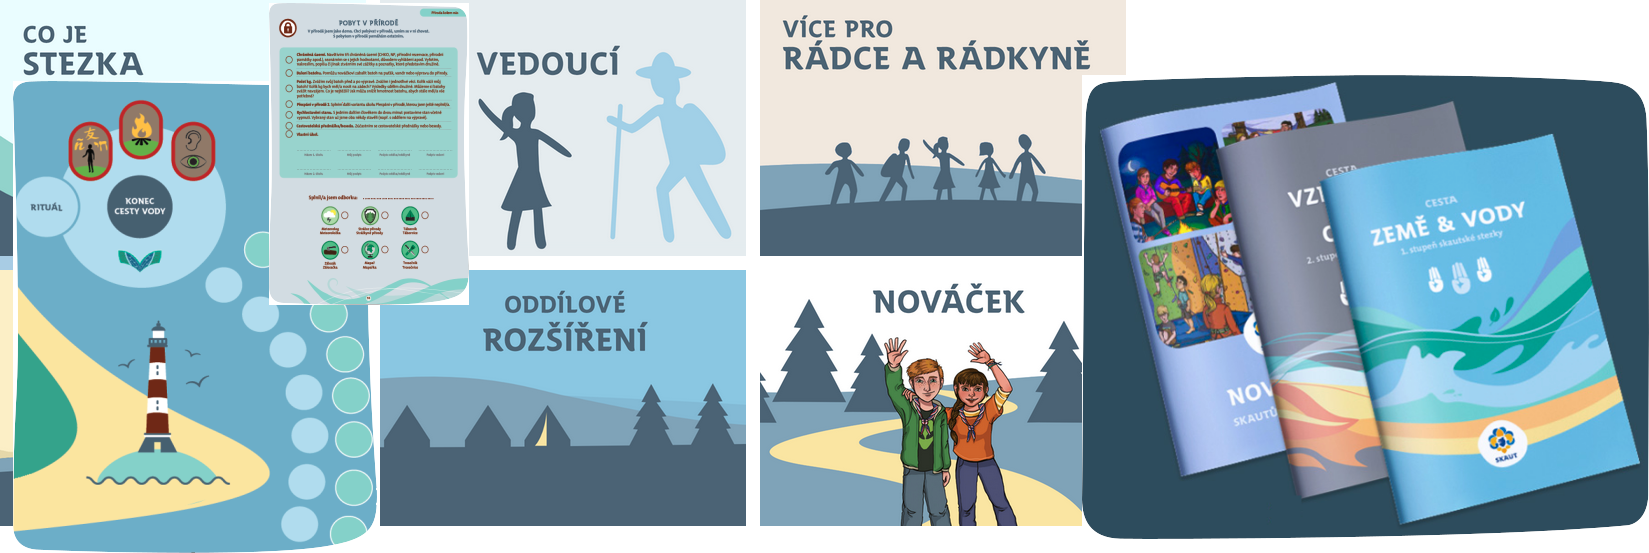
\includegraphics[height=6cm]{stezka.png}
\end{center}
\end{frame}

\begin{frame}{Stezka nejsou jen 4~sešity}
\begin{multicols}{2}
\begin{itemize}
\item Propracovaný systém nástrojů a~motivačních prvků
\item Prostředek k~dosahování výchovných cílů
\item Hlavní průvodce na cestě osobního rozvoje
\item Vede k~osobnímu rozvoji
\item Obsahuje program zajímavý pro dnešní děti
\item Má atraktivní a~srozumitelnou formu
\item Čtyři stupně (věkové kategorie) --- čtyři živly
\end{itemize}
\columnbreak
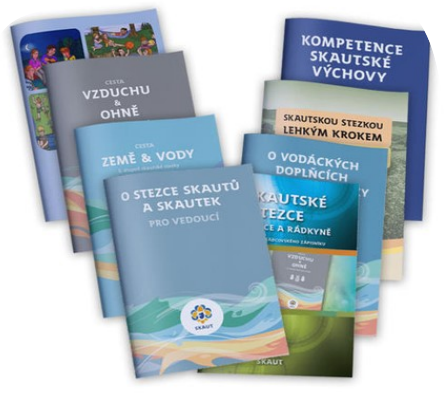
\includegraphics[height=7cm]{stezky.png}
\end{multicols}
\end{frame}

\begin{frame}{Nováček --- pro začátek}
\begin{multicols}{2}
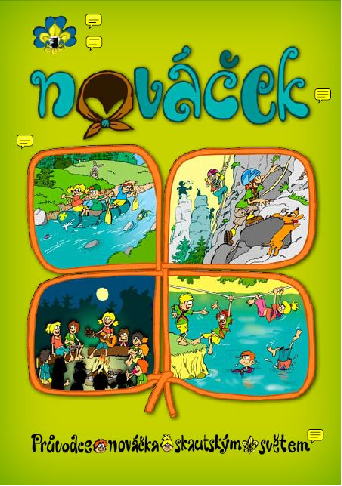
\includegraphics[height=7cm]{novacek.png}
\columnbreak
\begin{itemize}
\item Uvede nováčka do oddílu
\item Zábavná forma
\item Seznámí se skautingem a~vším, co k~němu patří
\item Oddílové doplňky --- variabilní
\item Varianty pro světlušky, vlčata, vodní i~suchozemské skauty a~skautky
\item \href{http://krizovatka.skaut.cz/oddil/program/skauti-skautky/skauti-skautky-stezky/novacek}{Ke stažení v~různých variantách}
\end{itemize}
\end{multicols}
\end{frame}

\begin{frame}{Postavy a~pomocníci --- plnění je zábava}
\begin{multicols}{2}
\begin{itemize}
\item Symbolický rámec dobrodružného světa
\item Na cestu si dítě jednu z~postav vybere jako průvodce, pomocníka
\item Za každou splněnou oblast získám pomocníka
\item Existuje (a~je \href{http://krizovatka.skaut.cz/oddil/program/skauti-skautky/skauti-skautky-stezky/skauti-skautky-stezky-stezky}{ke stažení}) i~varianta bez fantasy („turistická“) --- oddíl si může vytvořit vlastní symbolický rámec
\end{itemize}
\columnbreak
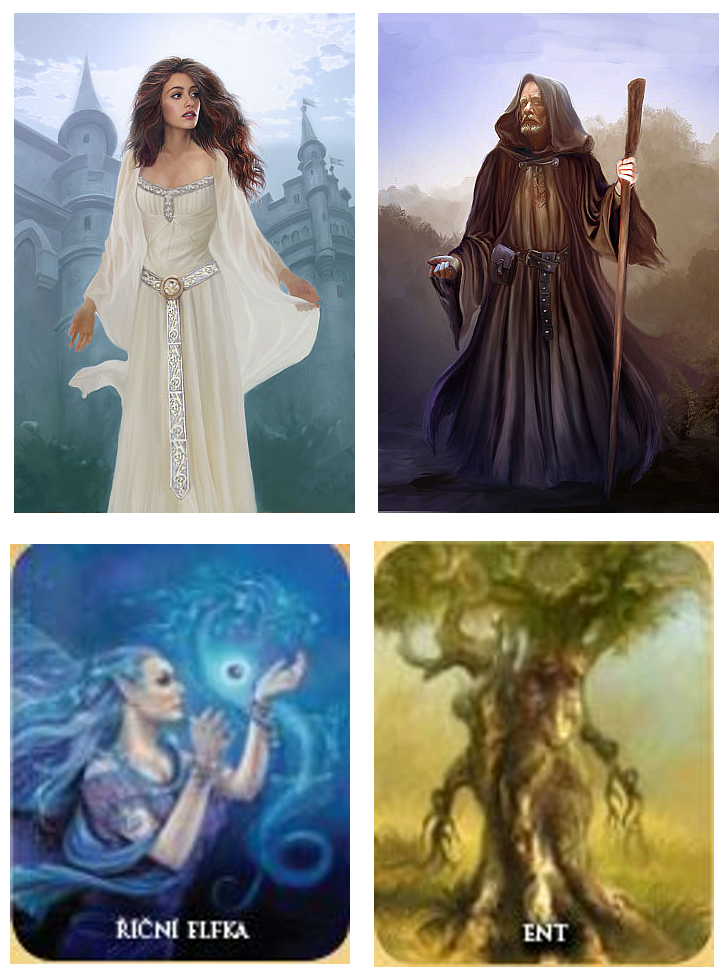
\includegraphics[height=6.5cm]{postavy.png}
\end{multicols}
\end{frame}

\begin{frame}{Sacculus}
\begin{multicols}{2}
\begin{itemize}
\item Motivační karetní hra
\item Doplněk ke stezce
\item 9~základních karet a~kamínky
\item 27 speciálních karet pro každý stupeň
\item Za splněný bod stezky 1~speciální karta
\begin{itemize}
 \item Čím více bodů stezky splní, tím silnější je hráč
\end{itemize}
\item V~principu podobné kartám Magic
\item \href{http://krizovatka.skaut.cz/oddil/program/skauti-skautky/skauti-skautky-stezky/skauti-skautky-stezky-sacculus}{Podrobnosti on-line}
\end{itemize}
\columnbreak
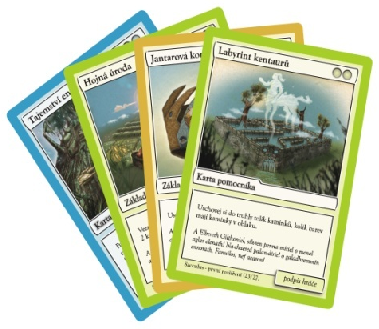
\includegraphics[height=4cm]{sacculus.png}
\end{multicols}
\end{frame}

\begin{frame}{Nášivky za splnění stupňů stezky --- motivace na začátku}
\begin{itemize}
\item Nášivka na začátku plnění stupně
 \begin{itemize}
 \item Vyjadřuje důvěru, že dítě daný stupeň splní
 \end{itemize}
\item Závěrečný bílý krystal až po splnění všech stupňů
\end{itemize}
\begin{center}
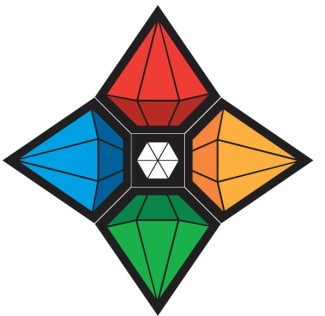
\includegraphics[height=4cm]{kameny.png}
\end{center}
\end{frame}

\begin{frame}{Skautské výzvy --- něco velkého, nevšedního}
\begin{multicols}{2}
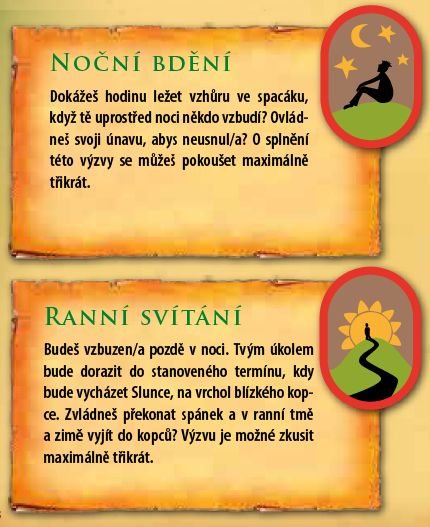
\includegraphics[height=6.1cm]{vyzvy.png}
\begin{itemize}
\item Po splnění stupně privilegovaná možnost plnit si jednu výzvu
 \begin{itemize}
 \item Noční bdění
 \item Ranní svítání
 \item Výsadek
 \item Noční návrat
 \item Tři orlí pera
 \item Dva dny bez ničeho
 \item 24 hodin na stromech
 \end{itemize}
 \item \href{http://krizovatka.skaut.cz/oddil/program/skauti-skautky/skauti-skautky-stezky/skauti-skautky-stezky-vyzvy}{Kompletní seznam je on-line}
\end{itemize}
\end{multicols}
\end{frame}

\begin{frame}{Výhody stezky}
\begin{itemize}
\item Všestrannost, rozličnost a~osobní zapojení
\item Stezka je vodítkem pro vytváření celoročního programu
\item Stezka umožňuje snadné přizpůsobení oddílu
\item Propracovaný nástroj osobního rozvoje
\item Zatraktivnění programu
\end{itemize}
\begin{center}

\includegraphics[height=4.5cm]{im-possible_m.png}
\end{center}
\end{frame}

\begin{frame}{Pravidla a~plnění stezky}
\begin{itemize}
\item Výběr aktivit
 \begin{itemize}
 \item Některé jsou povinné
 \item Vybírá se po konzultaci s~vedoucím (neplní se všechny)
 \item Lze je plnit v~libovolném pořadí
 \item Aktivitu lze upravit, vymyslet,~\ldots
 \end{itemize}
\item Kdo hodnotí
 \begin{itemize}
 \item Dítě a~dvě další osoby (vedoucí, rádce, rodič, externí odborník,~\ldots)
 \end{itemize}
\item Hodnocení
 \begin{itemize}
 \item Rozdíl 1. a~2. stupeň a~3. a~4.
 \end{itemize}
\item Plnění
 \begin{itemize}
 \item Přímé plnění
 \item Nepřímé plnění
 \item Přímé plnění s~přípravou
 \item Pro některé body nejsou vhodné všechny způsoby
 \end{itemize}
\end{itemize}
\end{frame}

\begin{frame}{Stezka zdaleka není vše\ldots}
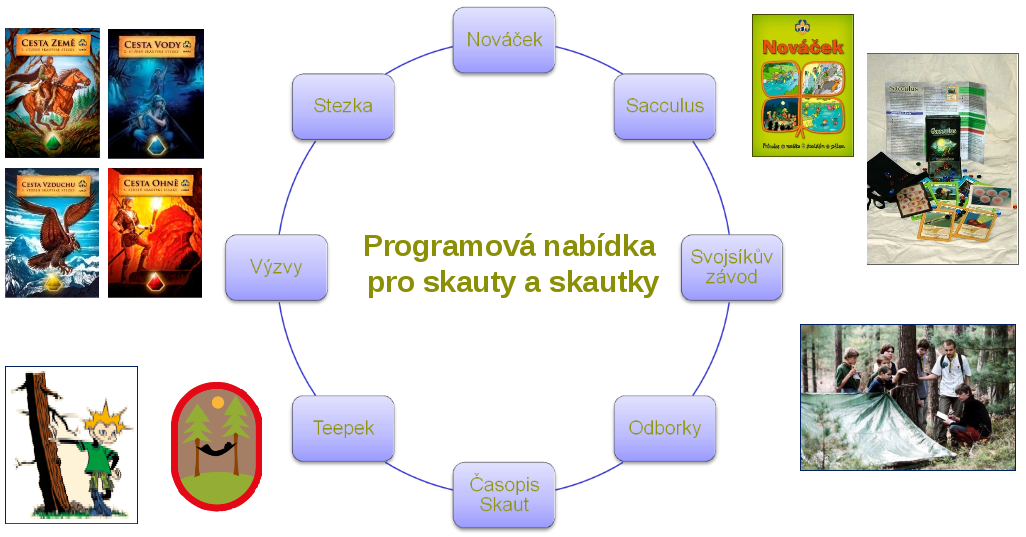
\includegraphics[width=\textwidth]{komplet.png}
\end{frame}

\section{Motivace}

\begin{frame}{Cíle a~zpětná vazba}
\begin{multicols}{2}
\begin{itemize}
\item Cíl musí být dostatečně podnětný, ale i~reálný
\item Měl by být součástí delšího plánu --- obecné (dlouhodobé) a~konkrétní (krátkodobé) cíle
\item Oddílová činnost musí být zábavná a~motivační, ale musí vést k~plnění výchovných cílů
\end{itemize}
\columnbreak
\begin{itemize}
\item Zpětná vazba musí být elektivní
\item Je třeba vyzdvihnout, co děti dělají dobře: i~malý pokrok je výhra
\item Co nás čeká a~čeho jsme dosáhli\ldots
\item Vyjádření uznání
 \begin{itemize}
 \item Formálně i~neformálně
 \item Upřímné, nefalšované
 \item Spravedlivá odměna
 \end{itemize}
\end{itemize}
\end{multicols}
Bez motivace (dospělých) to v~nevládní neziskové organizaci nejde\ldots~--- vedoucí a~další činovníci pro Junáka pracují ve svém volném čase.
\end{frame}

\begin{frame}{Oddílové motivační prostředky}
\begin{itemize}
\item Zapojení do celoroční, táborové hry --- veškerá činnost pak tvoří jeden logický celek
\item Symbolický rámec --- získání zvláštních schopností,~\ldots
\item Motivační scénky
\item Bodování (existují názory pro i~proti jeho používání)
\item Mapa postupu členů v~plnění
\item Speciální odměny všeho druhu
\item Motivace samotným programem
 \begin{itemize}
 \item Program musí být zábavný
 \item Programy lze spojovat do projektů
 \end{itemize}
\item \textbf{Pozor na záměnu prostředku za cíl!})
 \begin{itemize}
 \item Není cílem hrát si na Indiány, ale hraní si na Indiány je \textit{prostředkem} k~plnění výchovných cílů (znalostních, dovednostních i~etických, vztahových, \ldots)
 \end{itemize}
\item Motivace samotným programem
\item \ldots
\end{itemize}
\end{frame}

\section{Závěr}

\begin{frame}{Junák dnes}
\begin{itemize}
 \item Nové jméno: \textbf{„Junák --- český skaut, z. s.“} (jedna ze změn vynucená novým občanským zákoníkem)
 \item Přes \textbf{50~000 členů} --- největší dětská organizace v~ČR, poslední léta setrvale rosteme (podrobnosti ve \href{http://www.skaut.cz/skauting/o-skautingu}{výroční zprávě})
 \item \textbf{Strategie 2022} --- kam chceme dojít, podrobnosti \href{http://krizovatka.skaut.cz/organizace/strategie}{na Křižovatce} a~\href{http://strategie.skauting.cz/}{http://strategie.skauting.cz/}
 \item Konkurenční prostředí
 \begin{itemize}
  \item Vzniklo několik dalších skautských organizací
  \item Plno možností trávení volného času
  \item My toho po dětech hodně chceme
  \item „Je to levné, tak to musí být špatné“
 \end{itemize}
 \item Výzvy
 \begin{itemize}
  \item Neztratit zájem dětí a~udržet si své cíle
  \item Být respektovanou organizací s~odborným a~morálním kreditem
  \item Získat peníze na činnost
 \end{itemize}
\end{itemize}
\end{frame}

\begin{frame}{Metodická podpora vedoucích}
\begin{itemize}
\item Weby \href{http://krizovatka.skaut.cz/oddil/program}{http://krizovatka.skaut.cz/oddil/program} a~\href{http://krizovatka.skaut.cz/organizace/vzdelavani/vzdelavaci-system}{http://krizovatka.skaut.cz/organizace/vzdelavani/vzdelavaci-system}
\item Metodické příručky (za $\sim$30--50~Kč nebo \href{http://www.obchod.skaut.cz/index.php?tpl=&_artperpage=99&cl=alist&searchparam=&cnid=701}{zdarma elektronicky})
\item Semináře (i~na  požádání)
\item Konzultace (potřebujete poradit?)
\item Přijímáme zpětnou vazbu --- celý proces je lidmi z~oddílů připomínkován a~testován
\end{itemize}
\begin{center}
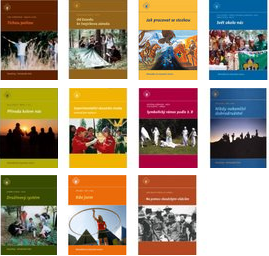
\includegraphics[width=4cm]{prirucky.png}
\end{center}
\end{frame}

\begin{frame}{Na čem právě pracujeme, co nás čeká v~brzké budoucnosti}
\begin{center}

\includegraphics[width=2cm]{lilie-cz.png}
\end{center}
\begin{itemize}
 \item Revize kompetencí a~stezek --- jak se osvědčily, co zlepšit
 \item Odborky a~další doplňky ke stezce
 \item Doplňky programu pro vlčata a~světlušky (mladší školní věk)
 \item Předškolní věk („benjamínci“), rodinný skauting, inkluzivní skauting pro znevýhodněné (nějak hendikepované, sociálně slabé, \ldots), lepší vzdělávání dospělých, \ldots
 \item Lepší zapojení oldskautů, lepší personalistika (neztrácet lidský potenciál) a~využití dostupných dat
 \item Stále být pro děti atraktivní a~neztratit nic z~cílů a~ideálů
 \item \ldots
\end{itemize}
\end{frame}

\begin{frame}{Další informace}
\begin{itemize}
\item Informace o~skautském výchovném programu: \href{http://krizovatka.skaut.cz/organizace/vzdelavani/vzdelavaci-system}{http://krizovatka.skaut.cz/organizace/vzdelavani/vzdelavaci-system} a~\href{http://krizovatka.skaut.cz/oddil/program}{http://krizovatka.skaut.cz/oddil/program}
 \begin{itemize}
 \item Materiály ke stažení
 \item Informace o~seminářích, kurzech,~\ldots
 \item Databáze programů
 \item Řada dalších informací\ldots
 \end{itemize}
\item Web pro veřejnost: \href{http://www.skaut.cz/}{http://www.skaut.cz/}
\item Časopisy elektronicky: \href{http://casopisy.skaut.cz/}{http://casopisy.skaut.cz/}
\item Kniha \textbf{Skautské století} (Roman Šantora, Václav Nosek, Slavomil Janov a~Václav Dostál, TDC a~Mladá fronta, 2012), \href{http://www.skautskyinstitut.cz/}{http://www.skautskyinstitut.cz/}
\item Budete-li mít v~budoucnu dotazy, klidně se mi ozvěte a~zeptejte se: \href{mailto:zeisek@natur.cuni.cz}{zeisek@natur.cuni.cz}, \href{http://trapa.cz/cs/contact}{http://trapa.cz/cs/contact}, \href{http://krizovatka.skaut.cz/organizace/instituce-organy/ustredni-organy/odbory/odbory-ekoodbor}{http://skaut.cz/eko}
\end{itemize}
\end{frame}

\begin{frame}{Děkuji za pozornost\ldots}
\begin{center}
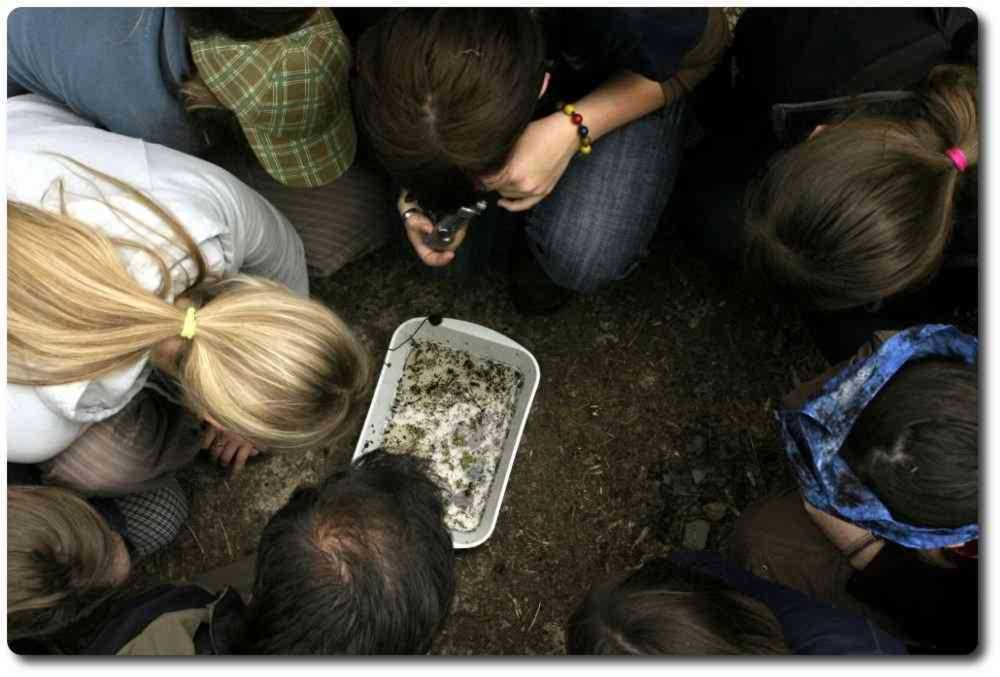
\includegraphics[height=6cm]{zaver.jpg}
\end{center}
\begin{flushright}
\begin{large}\ldots otázky?\end{large}
\end{flushright}
\end{frame}

\end{document}
